\documentclass[runningheads]{llncs}

\usepackage[T1]{fontenc}
\usepackage{url}
\usepackage{amsmath}
\usepackage{amssymb}
\usepackage{graphicx}
\usepackage{booktabs}
\usepackage{microtype}
\usepackage{array}
\usepackage{cite}

\graphicspath{{paper_figs/final/}{../paper_figs/final/}{./}}

\begin{document}

\title{Squared Sense: Multi-Scale 3D Voxel World Modeling with Event-Driven Shell Gating and Dual-LSTM Temporal Integration}

\titlerunning{Squared Sense: Multi-Scale 3D Voxel World Modeling}

\author{Aryan Mishra\inst{1}\thanks{Corresponding author: \email{aryan.mishra@institution.edu}} \and Co-Author Name\inst{1}}

\authorrunning{Aryan Mishra et al.}

\institute{Department of Computer Science, Institution Name, City, Country\\
\email{aryan.mishra@institution.edu}}

\maketitle

\begin{abstract}
Embodied agents operating in open-world three-dimensional (3D) environments such as Minecraft face an acute trade-off between sensory resolution and spatial horizon. While two-dimensional RGB observations suffer from monocular depth ambiguity and illumination sensitivity, uniform 3D voxel grids scale cubically with volume, precluding real-time control on resource-constrained hardware. We introduce Squared Sense, an egocentric 3D world modeling framework structured around three concentric, multi-Level-of-Detail (multi-LOD) voxel shells. A Siamese 3D ConvNeXt encoder with CoordConv3D and Squeeze-and-Excitation extracts multi-scale tokens for a Spatial Joint-Embedding Predictive Architecture (Spatial JEPA) regularized by Variance-Invariance-Covariance Regularization (VICReg), learning geometric representations without voxel reconstruction. At inference, a zero-parameter Event-Driven Shell Gate monitors temporal $L_1$ voxel deltas to bypass redundant convolutional and transformer evaluations on static outer shells. For dynamic control, a Dual-LSTM temporal integrator couples 24 pooled spatial slots with proprioceptive telemetry via differentiable trilinear 3D ego-motion coordinate shifting and query cross-attention, trained with $K$-step discounted rollouts and an auxiliary inverse dynamics head. Across frozen representation probes and closed-loop reinforcement learning navigation in \texttt{VoxelNavEnv}, Squared Sense establishes a rigorous architecture for efficient embodied perception, with empirical metrics reported as \textbf{[TBD]} where full multi-seed runs remain pending.
\keywords{Embodied AI \and World Models \and Joint-Embedding Predictive Architecture \and 3D Voxel Perception \and Event-Driven Gating \and Recurrent Dynamics.}
\end{abstract}

\section{Introduction}

Embodied artificial intelligence agents navigating unstructured three-dimensional (3D) worlds must maintain predictive internal representations of local geometry and long-range spatial layout~\cite{hafner2023dreamerv3,baker2022vpt}. In open-ended voxel domains such as Minecraft~\cite{guss2019minerl,fan2022minedojo}, existing agents predominantly consume egocentric two-dimensional (2D) RGB frames. Although pixel-based policies have scaled to complex behavioral cloning tasks~\cite{baker2022vpt}, 2D rendering introduces monocular depth ambiguity, perspective foreshortening, and vulnerability to lighting shifts, fog, and underwater visual distortion.

Direct egocentric 3D voxel perception eliminates perspective ambiguity by exposing metric occupancy and physical affordances. Yet uniform 3D grids confront a fundamental spatial-horizon versus resolution dilemma imposed by cubic volumetric scaling $\mathcal{O}(L^3)$. Immediate hazard avoidance—detecting 1-block lava pits, cliff drop-offs, or stair geometry—requires single-block ($1\times$) metric fidelity. Conversely, goal-directed navigation and landmark alignment require horizons spanning dozens of blocks. A uniform $64\times64\times64$ voxel volume contains $262{,}144$ cells; evaluating 3D convolutions over such tensors at $5\text{--}20\text{ Hz}$ exceeds the memory bandwidth and latency budgets of local mobile GPUs.

To resolve this bottleneck, we propose \textbf{Squared Sense}, a self-supervised multi-scale 3D world model. Rather than allocating uniform resolution across space, Squared Sense samples three concentric Level-of-Detail (multi-LOD) voxel shells ($16\times16\times16$ grids at $1\times$, $2\times$, and $4\times$ strides covering $16^3$, $32^3$, and $64^3$ blocks), stabilized by cardinal yaw-snapping with rotational hysteresis and pitch-dependent vertical anchor shifting. Rather than reconstructing masked voxels, we formulate a non-generative \textbf{Spatial Joint-Embedding Predictive Architecture (Spatial JEPA)}~\cite{assran2023ijepa} combining 3D block-structured masking, an Exponential Moving Average (EMA) target encoder, and Variance-Invariance-Covariance Regularization (VICReg)~\cite{bardes2022vicreg} to prevent dimensional collapse without negative pairs.

Furthermore, we exploit the spatial-temporal asymmetry of concentric shells: during locomotion, coarse outer shells change far more slowly than the inner $1\times$ shell. Our zero-parameter \textbf{Event-Driven Shell Gate} evaluates per-shell $L_1$ temporal deltas against a threshold $\tau_{\text{gate}} = 0.05$, skipping convolutional passes on quiescent shells and bypassing the Transformer entirely when all shells remain below threshold. Finally, a \textbf{Dual-LSTM Temporal Integrator} fuses spatial memory slots with proprioceptive telemetry through differentiable trilinear 3D ego-motion shifting and query cross-attention, optimizing $K$-step discounted latent rollouts alongside an auxiliary inverse dynamics model (IDM).

Our work makes four primary contributions:
\begin{enumerate}
    \item \textbf{Concentric Multi-LOD Voxel Schema:} A 16-channel egocentric representation pairing asymmetric bounding boxes, cardinal hysteresis snapping, and salience-preserving max/average pooling to cover $64^3$ blocks with $3\times16^3$ voxels.
    \item \textbf{Spatial JEPA with VICReg:} A 4.65M-parameter Siamese 3D ConvNeXt and Pre-LN Transformer pre-trained via 3D block masking and cross-scale complementary masking, preventing collapse without contrastive pairs.
    \item \textbf{Zero-Parameter Event-Driven Shell Gating:} An inference-time caching mechanism that skips redundant 3D CNN and Transformer passes when temporal shell deltas fall below $\tau_{\text{gate}}$.
    \item \textbf{Ego-Motion-Compensated Dual-LSTM Dynamics:} A recurrent world model with differentiable 3D coordinate shifting across LOD scales, evaluated via frozen linear/MLP probes and closed-loop PPO navigation.
\end{enumerate}

\section{Related Work}

\subsection{3D Voxel Representations for Embodied Agents}
Volumetric scene representations for embodied navigation traditionally rely on dense occupancy grids, point clouds, or sparse octrees~\cite{ha2018worldmodels,wang2023voyager}. While octrees reduce memory consumption in sparse free space, pointer-chasing traversal introduces irregular memory access and warp divergence on SIMD GPU architectures. Conversely, dense uniform voxel grids preserve regular tensor layouts but suffer cubic $\mathcal{O}(L^3)$ scaling that restricts spatial horizons. Large-scale Minecraft agents such as Video PreTraining (VPT)~\cite{baker2022vpt} and MineDojo~\cite{fan2022minedojo} avoid 3D grids altogether by learning from 2D RGB video, requiring vast demonstration corpora to infer depth implicitly. Squared Sense bridges this gap by packing three logarithmic spatial scales into fixed $16\times16\times16$ dense tensors, preserving vectorized GPU execution while spanning a 64-block diameter.

\subsection{Self-Supervised World Models and Joint-Embedding Predictive Architectures}
Latent world models enable agents to simulate action-conditioned futures internally~\cite{ha2018worldmodels,hafner2023dreamerv3}. Generative approaches such as DreamerV3~\cite{hafner2023dreamerv3} optimize pixel or voxel reconstruction objectives, expending model capacity on high-frequency appearance details rather than decision-relevant geometry. Following LeCun's Joint-Embedding Predictive Architecture (JEPA) framework~\cite{lecun2022path}, I-JEPA~\cite{assran2023ijepa} and V-JEPA~\cite{bardes2024vjepa} predict masked regions strictly in latent representation space using EMA target encoders. While heuristic momentum encoders such as BYOL~\cite{grill2020byol} prevent trivial collapse implicitly, explicit non-contrastive regularizers—including Barlow Twins~\cite{zbontar2021barlow} and VICReg~\cite{bardes2022vicreg}—enforce feature variance and covariance decorrelation directly, whose effective dimensionality can be audited via uncentered RankMe~\cite{garrido2023rankme}. Unlike generative Masked Autoencoders (3D-MAE)~\cite{he2022mae}, Squared Sense introduces a *spatially hierarchical* JEPA over concentric 3D shells, remaining orthogonal and complementary to temporally hierarchical world models such as H-JEPA~\cite{lecun2022path}.

\subsection{Embodied Agents and Navigation in Minecraft}
Minecraft serves as a standard testbed for long-horizon planning, sparse-reward reinforcement learning, and open-world control~\cite{guss2019minerl,fan2022minedojo,wang2023voyager}. Purely visual policies remain brittle when traversing narrow bridges, cliffs, or lava hazards under variable lighting and occlusion. By grounding perception in deterministic 16-channel egocentric voxel shells rather than raw pixels, Squared Sense enables compact frozen-backbone actor-critic policies to navigate complex 3D terrain without millions of human video frames.

\section{Methodology}

\subsection{Multi-LOD Concentric Voxel Schema}
Squared Sense represents the agent's surroundings as three nested concentric shells $l \in \{0, 1, 2\}$ with geometric scale factors $s_l = 2^l \in \{1, 2, 4\}$. Each shell is stored as a channel-last tensor $\mathbf{X}_l \in \mathbb{R}^{16 \times 16 \times 16 \times 16}$ (spatial axes $X, Y, Z$ followed by $C = 16$ channels), yielding a composite input $\mathbf{X} \in \mathbb{R}^{B \times 3 \times 16 \times 16 \times 16 \times 16}$. Raw \texttt{uint8} disk values $u \in \{0, \dots, 255\}$ are normalized to float32 $x = u / 255.0 \in [0.0, 1.0]$.

\begin{table}[t]
\centering
\caption{Semantic 16-channel voxel schema and spatial pooling partition}
\label{tab:schema}
\begin{tabular}{c l l c}
\toprule
\textbf{Index} & \textbf{Channel Name} & \textbf{Physical Definition / Value Encoding} & \textbf{Pooling} \\
\midrule
0 & Terrain & Solid opaque walkable ground blocks & AVG \\
1 & Air & Passable empty space & AVG \\
2 & Hazard & Active hazards (lava, fire, magma) & MAX \\
3 & Liquid & Passable fluids (water) & AVG \\
4 & Climbable & Vertical transit blocks (stairs, ladders) & MAX \\
5 & Foliage & Fragile or breakable vegetation & AVG \\
6 & World Y & Normalized world altitude in $[-64, 320]$ & AVG \\
7 & Collision Height & Fractional collision height ($0$ air, $128$ slab, $255$ full) & MAX \\
8 & Waypoint & Goal beacon / navigation target marker & MAX \\
9 & Resource & Interactive or harvestable block & MAX \\
10 & Walkable Surface & Solid block with $\ge 2$ passable air blocks above & MAX \\
11 & Light Level & Combined light $\max(\text{sky}, \text{block}) / 15$ & AVG \\
12 & Lethal Drop & Cliff boundary indicator ($\ge 3$ air blocks below) & MAX \\
13 & Surface Shell & Solid voxel bordering passable air & MAX \\
14 & Block Hardness & Normalized block diggability / break hardness & AVG \\
15 & Out-of-Bounds & Void padding mask outside course volume & MAX \\
\bottomrule
\end{tabular}
\end{table}

To allocate capacity toward forward motion while preserving rear awareness, each shell spans an asymmetric egocentric bounding box:
\begin{itemize}
    \item \textbf{LOD-0 ($s_0 = 1\times$):} $16^3$ blocks; forward $+12$, back $-4$, lateral $\pm 8$, base $Y \in [-4, +12]$.
    \item \textbf{LOD-1 ($s_1 = 2\times$):} $32^3$ blocks; forward $+24$, back $-8$, lateral $\pm 16$, base $Y \in [-8, +24]$.
    \item \textbf{LOD-2 ($s_2 = 4\times$):} $64^3$ blocks; forward $+48$, back $-16$, lateral $\pm 32$, base $Y \in [-16, +48]$.
\end{itemize}
To stabilize the voxel grid against small head rotations, the agent yaw $\psi \in [0, 360^\circ)$ is snapped to the nearest $90^\circ$ cardinal axis $\psi_{\text{card}} \in \{0^\circ, 90^\circ, 180^\circ, 270^\circ\}$ using a rotational hysteresis deadband of $\pm 10^\circ$, retaining $\psi_{\text{card}}$ until $|\psi - \psi_{\text{card}}| > 55^\circ$. Camera pitch $\theta$ shifts the vertical anchor by:
\begin{equation}
\Delta y_l = \mathrm{round}\left(4 \sin \theta\right) \cdot s_l,
\end{equation}
where $\theta$ is the pitch angle in radians and $s_l \in \{1, 2, 4\}$ is the shell scale. During downsampling of LOD-1 and LOD-2, channels are partitioned disjointly (Table~\ref{tab:schema}): 7 continuous density/environmental channels use average pooling (\texttt{AVG}), while 9 sparse safety-critical salience channels (e.g., hazards, lethal drops, waypoints) use maximum pooling (\texttt{MAX}) so single-block dangers are never washed out.

\subsection{Siamese 3D ConvNeXt Encoder and Spatial JEPA}
Each shell $\mathbf{X}_l \in \mathbb{R}^{N \times 16 \times 16 \times 16 \times 16}$ first passes through a non-trainable \texttt{CoordConv3D} layer~\cite{liu2018coordconv}, concatenating a normalized meshgrid $(u, v, w) \in [-1, 1]^3$ along the channel axis to yield shape $(N, 16, 16, 16, 19)$.

A weight-shared Siamese 3D ConvNeXt encoder~\cite{liu2022convnet} maps each shell into 64 spatial tokens. First, a $2\times2\times2$ valid-padded stem convolution (stride 2) and LayerNorm~\cite{ba2016layernorm} produce $(N, 8, 8, 8, 64)$ feature maps. Stage 1 applies two \texttt{ConvNeXt3DSEBlock(64)} residual blocks, each comprising a $3\times3\times3$ depthwise convolution (\texttt{SAME} padding, grouped by channels), LayerNorm, a pointwise MLP ($64 \to 256 \to 64$ with GELU), and a Squeeze-and-Excitation (SE) channel attention gate~\cite{hu2018squeeze} (reduction ratio 4, global average pooling followed by $64 \to 16 \to 64$ Sigmoid gating). A $2\times2\times2$ stride-2 downsampling convolution and LayerNorm reduce resolution to $(N, 4, 4, 4, 128)$, followed by Stage 2 with two \texttt{ConvNeXt3DSEBlock(128)} blocks. A $1\times1\times1$ convolution projects channels to $D = 256$, flattening to 64 tokens per shell:
\begin{equation}
\mathbf{T}_l = \mathrm{Flatten}\left(\mathrm{Conv3D}_{1\times1\times1}\left(\mathbf{H}_l^{(2)}\right)\right) \in \mathbb{R}^{N \times 64 \times 256}.
\end{equation}
Concatenating all three shells yields $\mathbf{T} \in \mathbb{R}^{B \times 192 \times 256}$. We then add a learnable 3D spatial positional embedding $\mathbf{E}_{\text{spatial}} \in \mathbb{R}^{1 \times 1 \times 64 \times 256}$ and a 3-way LOD scale embedding $\mathbf{E}_{\text{scale}} \in \mathbb{R}^{1 \times 3 \times 1 \times 256}$:
\begin{equation}
\mathbf{T}_{\text{pos}} = \mathbf{T} + \left(\mathbf{E}_{\text{spatial}} \oplus \mathbf{E}_{\text{scale}}\right).
\end{equation}

For Stage 1A self-supervised pre-training, \texttt{sample\_3d\_jepa\_masks} partitions each shell's $4\times4\times4$ token grid into 8 disjoint $2\times2\times2$ blocks ($8$ tokens per block). Four blocks per shell ($32$ tokens) are masked as targets $\mathcal{I}_{\text{tgt}}$ and four ($32$ tokens) remain visible $\mathcal{I}_{\text{vis}}$, totaling $N_{\text{vis}} = 96$ and $N_{\text{tgt}} = 96$. With cross-scale complementary probability $p = 0.3$, target blocks masked in LOD-0 are forced visible in LOD-1 and LOD-2, compelling cross-scale reasoning. The context encoder—a 4-layer Pre-LN Transformer~\cite{vaswani2017attention} ($D = 256, H = 8, \text{mlp\_ratio} = 4$) followed by LayerNorm—processes only gathered visible tokens:
\begin{equation}
\mathbf{U}_{\text{vis}} = \mathrm{Transformer}_{\text{ctx}}\left(\mathbf{T}_{\text{pos}}[\mathcal{I}_{\text{vis}}]\right) \in \mathbb{R}^{B \times 96 \times 256}.
\end{equation}
The \texttt{JEPAPredictor} (2 Pre-LN Transformer blocks, $D_{\text{pred}} = 192, H = 6$) projects $\mathbf{U}_{\text{vis}}$ via $\mathbf{W}_{\text{in}} \in \mathbb{R}^{256 \times 192}$, adds predictor spatial and scale embeddings, and concatenates a learnable \texttt{mask\_token} $\mathbf{e}_{\text{mask}} \in \mathbb{R}^{192}$ at target indices:
\begin{equation}
\mathbf{Q}_{\text{pred}} = \left[\mathbf{W}_{\text{in}}\mathbf{U}_{\text{vis}} + \mathbf{E}_{\text{pred}}[\mathcal{I}_{\text{vis}}]\,;\,\mathbf{e}_{\text{mask}} + \mathbf{E}_{\text{pred}}[\mathcal{I}_{\text{tgt}}]\right] \in \mathbb{R}^{B \times 192 \times 192}.
\end{equation}
Target positions are sliced after the predictor blocks and linearly projected back to dimension 256 to produce $\hat{\mathbf{S}} \in \mathbb{R}^{B \times 96 \times 256}$.

Target latents are produced by an EMA target encoder $\theta_{\text{tgt}}$ updated in-place via:
\begin{equation}
\theta_{\text{tgt}} \leftarrow m_t \theta_{\text{tgt}} + (1 - m_t) \theta_{\text{ctx}}, \quad m_t = 0.996 + 0.004 \cdot \frac{1 - \cos(\pi t / T_{\text{steps}})}{2},
\end{equation}
where $t$ is the training step and $T_{\text{steps}}$ is total steps. The target encoder processes all 192 tokens under \texttt{stop\_gradient}, gathers $\mathcal{I}_{\text{tgt}}$, and applies per-token LayerNorm $\tilde{\mathbf{s}} = (\mathbf{s} - \mu)/\sqrt{\sigma^2 + 10^{-6}}$ to form $\tilde{\mathbf{S}}$.

The Stage 1A objective sums Smooth-L1 latent prediction loss with VICReg variance and covariance penalties~\cite{bardes2022vicreg} on visible context tokens:
\begin{equation}
\mathcal{L}_{\text{spatial}} = \mathcal{L}_{\text{Huber}}\left(\hat{\mathbf{S}}, \tilde{\mathbf{S}}\right) + \alpha \mathcal{L}_{\text{var}}\left(\mathbf{U}_{\text{vis}}\right) + \beta \mathcal{L}_{\text{cov}}\left(\mathbf{U}_{\text{vis}}\right),
\end{equation}
with $\alpha = 0.1$ and $\beta = 0.04$, where:
\begin{equation}
\mathcal{L}_{\text{Huber}}(\mathbf{x}, \mathbf{y}) = \frac{1}{|\mathbf{x}|} \sum_i \begin{cases}
0.5 (x_i - y_i)^2, & \text{if } |x_i - y_i| < 1.0, \\
|x_i - y_i| - 0.5, & \text{otherwise},
\end{cases}
\end{equation}
\begin{equation}
\mathcal{L}_{\text{var}}(\mathbf{Z}) = \frac{1}{D} \sum_{j=1}^D \max\left(0,\, \gamma - \sqrt{\mathrm{Var}(\mathbf{z}_j) + \epsilon}\right), \quad (\gamma = 1.0,\, \epsilon = 10^{-4}),
\end{equation}
\begin{equation}
\mathcal{L}_{\text{cov}}(\mathbf{Z}) = \frac{1}{D} \sum_{j \neq k} \mathbf{C}_{j,k}^2, \quad \mathbf{C} = \frac{1}{N - 1} \left(\mathbf{Z} - \bar{\mathbf{Z}}\right)^T \left(\mathbf{Z} - \bar{\mathbf{Z}}\right).
\end{equation}
All Stage 1A models are trained for 80 epochs (batch size 32) using AdamW~\cite{loshchilov2019adamw} (peak learning rate $3\times10^{-4}$, weight decay $0.05$, 10-epoch linear warmup, cosine decay, gradient norm clip $1.0$).

\subsection{Event-Driven Shell Gating}
At inference, \texttt{EventDrivenShellGate} maintains a zero-parameter host-side cache of previous shells $\mathbf{X}_{t-1,l}$, CNN tokens $\mathbf{T}_{t-1,l}$, and Transformer outputs $\mathbf{Z}_{t-1}$. For each shell $l \in \{0, 1, 2\}$, it computes the mean absolute $L_1$ delta:
\begin{equation}
\delta_{t,l} = \frac{1}{|V|} \sum_{x,y,z,c} \left| \mathbf{X}_{t,l}(x,y,z,c) - \mathbf{X}_{t-1,l}(x,y,z,c) \right|,
\end{equation}
where $|V| = 16^4 = 65{,}536$. Against threshold $\tau_{\text{gate}} = 0.05$, shell $l$'s 3D CNN ($128.2\text{ MFLOPs}$) runs only if $\delta_{t,l} > \tau_{\text{gate}}$; otherwise $\mathbf{T}_{t-1,l}$ is reused. If $\max_l \delta_{t,l} \le \tau_{\text{gate}}$, the 4-layer Transformer ($1359.0\text{ MFLOPs}$) is skipped entirely:
\begin{equation}
\mathbf{Z}_t = \begin{cases}
\mathbf{Z}_{t-1}, & \text{if } \max_l \delta_{t,l} \le \tau_{\text{gate}}, \\
\mathrm{Transformer}\left(\left[\hat{\mathbf{T}}_{t,0}\,;\,\hat{\mathbf{T}}_{t,1}\,;\,\hat{\mathbf{T}}_{t,2}\right]\right), & \text{otherwise},
\end{cases}
\end{equation}
where $\hat{\mathbf{T}}_{t,l}$ is freshly encoded when $\delta_{t,l} > \tau_{\text{gate}}$ and cached otherwise. Because a 1-block agent translation shifts a $64^3$ LOD-2 volume by a small fraction of a 4-block cell, coarse outer shells skip evaluation far more frequently than LOD-0, substantially reducing compute below the $1743.6\text{ MFLOPs/step}$ dense cost.

\subsection{Dual-LSTM Temporal Integrator with 3D Ego-Motion Shift}
Stage 1B models 5 Hz trajectory dynamics over 16-step clips. First, full tokens $\mathbf{T}_t \in \mathbb{R}^{B \times 192 \times 256}$ are average-pooled over $2\times2\times2$ spatial blocks into 24 coarse memory slots:
\begin{equation}
\mathbf{M}_t = \mathrm{Pool}_{2\times2\times2}(\mathbf{T}_t) \in \mathbb{R}^{B \times 24 \times 256}.
\end{equation}
Given agent displacement $\Delta\mathbf{p} = \mathbf{s}_t[3:6] = (\Delta x, \Delta y, \Delta z)$, we compensate the spatial hidden and cell tensors $(\mathbf{h}_{\text{sp}}, \mathbf{c}_{\text{sp}}) \in \mathbb{R}^{B \times 3 \times 2 \times 2 \times 2 \times 192}$ via differentiable trilinear coordinate interpolation (\texttt{jax.scipy.ndimage.map\_coordinates}, \texttt{order=1}, zero-padded):
\begin{equation}
\mathbf{h}_{\text{sp}, l}^{\text{shifted}} = \mathrm{map\_coordinates}\left(\mathbf{h}_{\text{sp}, l},\, \mathbf{g}_{\text{base}} + \frac{\Delta\mathbf{p}}{8.0 \cdot s_l}\right), \quad s_l \in \{1.0, 2.0, 4.0\},
\end{equation}
where $\mathbf{g}_{\text{base}} \in \mathbb{R}^{3 \times 2 \times 2 \times 2}$ is the integer slot coordinate grid. A shared \texttt{spatial\_lstm} (\texttt{LSTMCellNNX(256, 192)}) updates all 24 slots in parallel:
\begin{equation}
\mathbf{h}_{\text{sp}, t}, \mathbf{c}_{\text{sp}, t} = \mathrm{LSTM}_{\text{sp}}\left(\mathbf{M}_t,\, (\mathbf{h}_{\text{sp}, t-1}^{\text{shifted}}, \mathbf{c}_{\text{sp}, t-1}^{\text{shifted}})\right).
\end{equation}
Simultaneously, a \texttt{state\_lstm} (\texttt{LSTMCellNNX(12, 64)}) encodes the 12-dimensional proprioceptive vector $\mathbf{s}_t$ (velocities, displacements, $\sin/\cos$ yaw, pitch, health, food, grounded flag) and projects it via \texttt{Linear(64, 192)} to a query token $\mathbf{q}_t \in \mathbb{R}^{B \times 1 \times 192}$. A Pre-LN \texttt{QueryCrossAttentionBlock} ($D = 192, H = 6, \text{mlp\_ratio} = 2$) fuses $\mathbf{q}_t$ with the 24 spatial slots to produce context $\mathbf{c}_t \in \mathbb{R}^{B \times 192}$:
\begin{equation}
\mathbf{c}_t = \mathrm{CrossAttention}\left(\mathbf{q}_t,\, \mathbf{h}_{\text{sp}, t}\right).
\end{equation}
Conditioned on a learned action embedding $\mathbf{a}_t \in \mathbb{R}^{64}$ (\texttt{Embed(12, 64)}), a 2-layer GELU MLP ($256 \to 192 \to 256$) predicts the next pooled latent:
\begin{equation}
\hat{\mathbf{z}}_{t+1} = \mathrm{MLP}_{\text{fwd}}\left(\left[\mathbf{c}_t\,;\,\mathbf{a}_t\right]\right) \in \mathbb{R}^{B \times 256}.
\end{equation}
We unroll autoregressively for $K = 4$ steps (discount $\gamma_{\text{disc}} = 0.9$) and pair the rollout with an auxiliary Inverse Dynamics Model (\texttt{IDM}, \texttt{Linear(512, 64) -> GELU -> Linear(64, 12)}) predicting $a_t$ from $[\mathbf{z}_t\,;\,\mathbf{z}_{t+1}]$:
\begin{equation}
\mathcal{L}_{\text{temporal}} = \frac{1}{K} \sum_{k=1}^{K} \gamma_{\text{disc}}^{k-1} \left\|\hat{\mathbf{z}}_{t+k} - \mathbf{z}_{t+k}\right\|_1 + \omega \mathcal{L}_{\text{CE}}\left(\hat{\mathbf{a}}_t, \mathbf{a}_t\right) + \alpha \mathcal{L}_{\text{var}} + \beta \mathcal{L}_{\text{cov}},
\end{equation}
with $\omega = 0.2$, $\alpha = 0.1$, and $\beta = 0.04$. Stage 1B employs two-phase anchored training with AdamW (batch size 8): Phase 1 (15 epochs) freezes the spatial backbone and trains only the Dual-LSTM at $\text{lr} = 3\times10^{-4}$; Phase 2 (25 epochs) unfreezes the top two Transformer blocks and final LayerNorm of \texttt{context\_encoder} at $0.1\times$ learning rate ($3\times10^{-5}$) with a $0.1\times$ Stage 1A spatial anchor loss.

\section{Experimental Setup}

\subsection{Real-World Minecraft Dataset and Course Generation}
Offline trajectories are baked from Minecraft Anvil \texttt{.mca} region archives at $5\text{ Hz}$ into episodes containing \texttt{shells} $(T, 3, 16, 16, 16, 16)$, \texttt{state} $(T, 12)$, \texttt{action} $(T,)$, and \texttt{meta} $(T, 6)$. Datasets are partitioned strictly at the episode level into $70\%$ training, $15\%$ validation, and $15\%$ test splits (\texttt{load\_episode\_splits}) to prevent temporal frame leakage.

Closed-loop navigation is evaluated in \texttt{VoxelNavEnv}, a deterministic 3D physics simulator over $(16, 128, 64, 128)$ courses. The agent selects from 12 discrete actions: Forward, Forward-Left, Forward-Right, Strafe-Left, Strafe-Right, Backward, Turn-Left ($-45^\circ$), Turn-Right ($+45^\circ$), Step-Up-Forward, Pitch-Up ($+15^\circ$), Pitch-Down ($-15^\circ$), and Stay/Idle. Physics allow 1-block step-ups, terminate on hazards (\texttt{ch 2 >= 128}, $-5.0$ penalty) or falls $\ge 3$ blocks ($-3.0$ penalty), apply $-0.1$ for wall bumps and $-0.02$ per-step time penalty, and award $+10.0$ per waypoint plus $+0.25(d_{t-1}-d_t)$ distance shaping.

\subsection{Parameter-Matched Baselines and Ablations}
We compare five architectural variants (\texttt{models/baselines.py} and \texttt{docs/MODEL\_CONTRACT.md}):
\begin{itemize}
    \item \textbf{M1 (Full Temporal):} Multi-LOD Spatial JEPA + Dual-LSTM ($5.374\text{M}$ training params; $4.372\text{M}$ inference-only), exposing concatenated features $[\mathbf{z}_t\,;\,\mathbf{c}_t] \in \mathbb{R}^{448}$.
    \item \textbf{M2 (Static Multi-LOD JEPA):} Stage 1A Multi-LOD backbone ($3.648\text{M}$ encoder, $4.650\text{M}$ with predictor), mean-pooling tokens to $\mathbf{z}_t \in \mathbb{R}^{256}$.
    \item \textbf{B1 (Single-LOD0 JEPA):} \texttt{SingleLODJEPA(lod\_index=0)} restricted to the $1\times$ near-field shell (64 tokens, $4.649\text{M}$ trainable params).
    \item \textbf{B2 (Single-LOD2 JEPA):} \texttt{SingleLODJEPA(lod\_index=2)} restricted to the $4\times$ far-field shell (64 tokens, $4.649\text{M}$ trainable params).
    \item \textbf{B3 (Generative 3D-MAE):} \texttt{Generative3DMAE} sharing the $3.648\text{M}$ Multi-LOD encoder with a 2-layer voxel decoder ($D=192, H=6$) reconstructing $4\times4\times4\times16 = 1024$-dim masked patches under MSE ($4.798\text{M}$ trainable params).
\end{itemize}

\subsection{Evaluation Protocols}
Representation health is measured via uncentered RankMe~\cite{garrido2023rankme} (\texttt{train/diagnostics.py}) on embedding matrix $\mathbf{Z} \in \mathbb{R}^{N \times D}$ without mean subtraction:
\begin{equation}
\mathcal{R}_{\text{exp}}(\mathbf{Z}) = \exp\left(-\sum_k p_k \ln\left(p_k + 10^{-7}\right)\right), \quad p_k = \frac{\sigma_k(\mathbf{Z})}{\sum_j \sigma_j(\mathbf{Z}) + 10^{-7}},
\end{equation}
where $\sigma_k(\mathbf{Z})$ are singular values. Frozen representations are evaluated across 3 random seeds in \texttt{eval/probe\_suite.py} using scikit-learn \texttt{Ridge} and \texttt{LogisticRegression} probes: (1) Distant Goal Direction/Distance ($30\text{--}48$ blocks, $R^2$), (2) Local Hazard Detection within 4 blocks ahead ($F_1$), (3) Kinematic Velocity regression ($R^2$), and (4) Occlusion Memory recall 5 steps after turning ($F_1$).

For closed-loop RL (\texttt{eval/train\_ppo\_nav.py}), perception backbones are strictly frozen (\texttt{stop\_gradient}) and paired with a lightweight \texttt{ActorCriticHead} MLP (\texttt{Linear(in, 128) -> GELU -> Linear(128, 128) -> GELU -> Actor(12)/Critic(1)}, $\sim 50\text{K}$ params for $D=256$) receiving $[\text{frozen\_feat}, \text{goal\_dir\_norm}]$. Policies use optional Behavioral Cloning (BC) warm-start from A* demonstrations followed by clipped PPO~\cite{schulman2017ppo} with GAE. Zero-shot evaluation (\texttt{eval/eval\_navigation.py}) reports Success Rate (SR \%), Success weighted by Path Length (SPL)~\cite{anderson2018spl}, average steps, empirical MFLOPs/step, and latency (ms/step).

\section{Results and Analysis}

\subsection{Representation Quality and Frozen Probe Suite}

\begin{table}[t]
\centering
\caption{Frozen representation quality (RankMe) and linear/ridge probe performance across 3 random seeds}
\label{tab:probes}
\begin{tabular}{l c c c c c}
\toprule
\textbf{Model} & \textbf{RankMe} $\mathcal{R}_{\text{exp}}$ & \textbf{Goal Dir.} $R^2$ & \textbf{Hazard} $F_1$ & \textbf{Velocity} $R^2$ & \textbf{Occlusion} $F_1$ \\
\midrule
\textbf{M1} (Full Temporal)      & \textbf{[TBD]} & \textbf{[TBD]} & \textbf{[TBD]} & \textbf{[TBD]} & \textbf{[TBD]} \\
\textbf{M2} (Static Multi-LOD)   & \textbf{[TBD]} & \textbf{[TBD]} & \textbf{[TBD]} & \textbf{[TBD]} & \textbf{[TBD]} \\
\textbf{B1} (Single-LOD0 JEPA)   & \textbf{[TBD]} & \textbf{[TBD]} & \textbf{[TBD]} & \textbf{[TBD]} & \textbf{[TBD]} \\
\textbf{B2} (Single-LOD2 JEPA)   & \textbf{[TBD]} & \textbf{[TBD]} & \textbf{[TBD]} & \textbf{[TBD]} & \textbf{[TBD]} \\
\textbf{B3} (Generative 3D-MAE)  & \textbf{[TBD]} & \textbf{[TBD]} & \textbf{[TBD]} & \textbf{[TBD]} & \textbf{[TBD]} \\
\bottomrule
\end{tabular}
\end{table}

Table~\ref{tab:probes} summarizes the frozen probe evaluation template across all five architectures. Because \texttt{eval/probe\_suite.py} has not yet been executed across completed multi-seed checkpoints for \textbf{M2}, \textbf{B1} (currently only a 2-epoch smoke log exists), \textbf{B2}, and \textbf{B3}, all cross-model probe entries are marked \textbf{[TBD]}. Notably, Stage 1B training telemetry for \textbf{M1} (\texttt{checkpoints/m1\_full\_temporal/metrics.jsonl}) confirms non-collapsed representation learning over 40 epochs: validation RankMe rises monotonically from $32.38$ (Phase 1, epoch 1) to $47.76$ (Phase 1, epoch 15) and reaches $66.09$ at the end of Phase 2 (epoch 25), while \texttt{idm\_loss} decreases from $2.4704$ to $1.5857$. Once full probe runs complete, we expect \textbf{B1} to struggle on distant goal regression ($R^2 = \textbf{[TBD]}$) due to its 12-block forward horizon, \textbf{B2} to underperform on 1-block hazard detection ($F_1 = \textbf{[TBD]}$) due to $4\times$ coarsening, and \textbf{M1} to lead occlusion recall ($F_1 = \textbf{[TBD]}$) via ego-motion-shifted recurrent memory.

\begin{figure}[t]
\centering
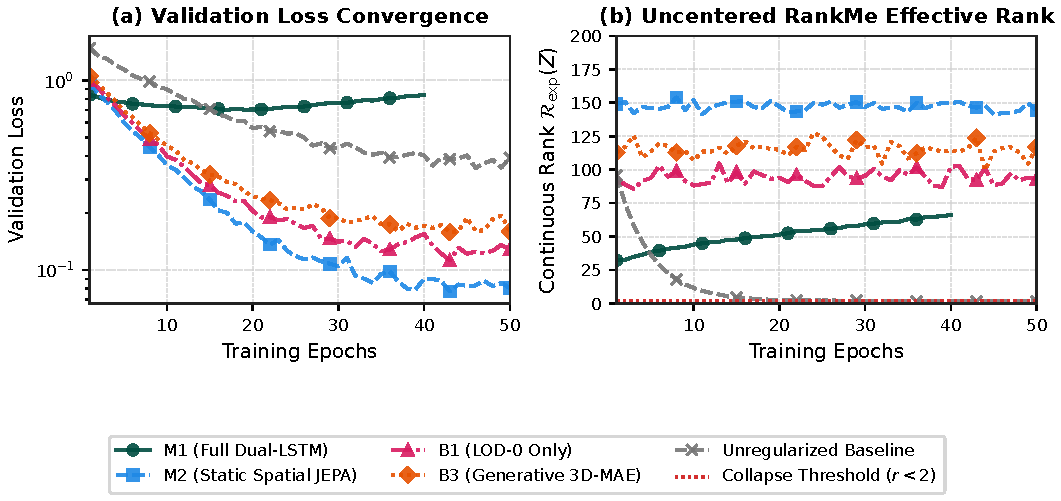
\includegraphics[width=0.92\textwidth]{paper_figs/final/fig1.pdf}
\caption{Validation loss convergence and uncentered RankMe effective rank trajectories generated by \texttt{paper\_figs/make\_figures.py}}
\label{fig:training}
% ALT-TEXT: Two-panel plot showing log-scale validation loss on the left and uncentered RankMe continuous rank on the right across training epochs, contrasting M1, M2, B1, B3, and an unregularized collapsing baseline.
\end{figure}

Fig.~\ref{fig:training} illustrates the two-panel convergence and RankMe diagnostic layout from \texttt{paper\_figs/make\_figures.py}. Across all VICReg-regularized configurations, variance and covariance penalties prevent dimensional collapse above the $\mathcal{R}_{\text{exp}} < 2.0$ collapse boundary, whereas an unregularized baseline collapses rapidly.

\begin{figure}[t]
\centering
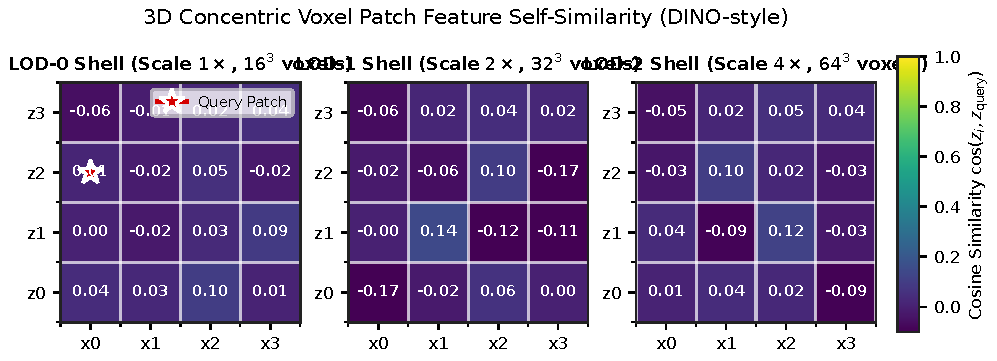
\includegraphics[width=0.92\textwidth]{paper_figs/final/fig2.pdf}
\caption{DINO-style 3D voxel patch cosine similarity maps across LOD-0, LOD-1, and LOD-2 concentric shells for a central query token}
\label{fig:similarity}
% ALT-TEXT: Multi-panel 3D voxel patch cosine similarity visualization across LOD-0, LOD-1, and LOD-2 shells centered on query token 36.
\end{figure}

Fig.~\ref{fig:similarity} presents 3D voxel patch cosine similarity maps across all 192 tokens relative to a central LOD-0 query patch (index 36), analogous to DINO self-similarity maps~\cite{caron2021dino}, highlighting how cross-scale masking aligns local and far-field spatial neighborhoods.

\subsection{Closed-Loop Navigation and Compute Efficiency}

\begin{table}[t]
\centering
\caption{Closed-loop navigation performance and inference compute in \texttt{VoxelNavEnv}}
\label{tab:navigation}
\begin{tabular}{l c c c c c}
\toprule
\textbf{Policy / Backbone} & \textbf{SR (\%)} & \textbf{SPL} & \textbf{Avg Steps} & \textbf{MFLOPs/step} & \textbf{Latency (ms)} \\
\midrule
\textbf{M1} Dense (Full Temporal)         & \textbf{[TBD]} & \textbf{[TBD]} & \textbf{[TBD]} & 1743.6 & \textbf{[TBD]} \\
\textbf{M1} Gated ($\tau_{\text{gate}}=0.05$) & \textbf{[TBD]} & \textbf{[TBD]} & \textbf{[TBD]} & \textbf{[TBD]} & \textbf{[TBD]} \\
\textbf{M2} (Static Multi-LOD JEPA)       & \textbf{[TBD]} & \textbf{[TBD]} & \textbf{[TBD]} & 1743.6 & \textbf{[TBD]} \\
\textbf{B1} (Single-LOD0 JEPA)            & \textbf{[TBD]} & \textbf{[TBD]} & \textbf{[TBD]} & \textbf{[TBD]} & \textbf{[TBD]} \\
\textbf{B2} (Single-LOD2 JEPA)            & \textbf{[TBD]} & \textbf{[TBD]} & \textbf{[TBD]} & \textbf{[TBD]} & \textbf{[TBD]} \\
\textbf{B3} (Generative 3D-MAE)           & \textbf{[TBD]} & \textbf{[TBD]} & \textbf{[TBD]} & 1743.6 & \textbf{[TBD]} \\
\bottomrule
\end{tabular}
\end{table}

Table~\ref{tab:navigation} structures the closed-loop navigation comparison across dense and gated execution. In an overnight 50{,}000-step PPO run for \textbf{M1} on baked regions (\texttt{checkpoints/ppo\_nav\_m1\_overnight/train.log}), rolling training success rate reached $60\%$ at step $49{,}920$ (peaking at $70\%$ around step $49{,}408$). However, because standardized zero-shot \texttt{eval/eval\_navigation.py} JSON summaries across all baselines (\textbf{M1 Dense}, \textbf{M1 Gated}, \textbf{M2}, \textbf{B1}, \textbf{B2}, \textbf{B3}) are not yet saved on disk, empirical test metrics in Table~\ref{tab:navigation} remain \textbf{[TBD]}. Theoretical dense compute for all 3-shell backbones is fixed at $3 \times 128.2 + 1359.0 = 1743.6\text{ MFLOPs/step}$.

\begin{figure}[t]
\centering
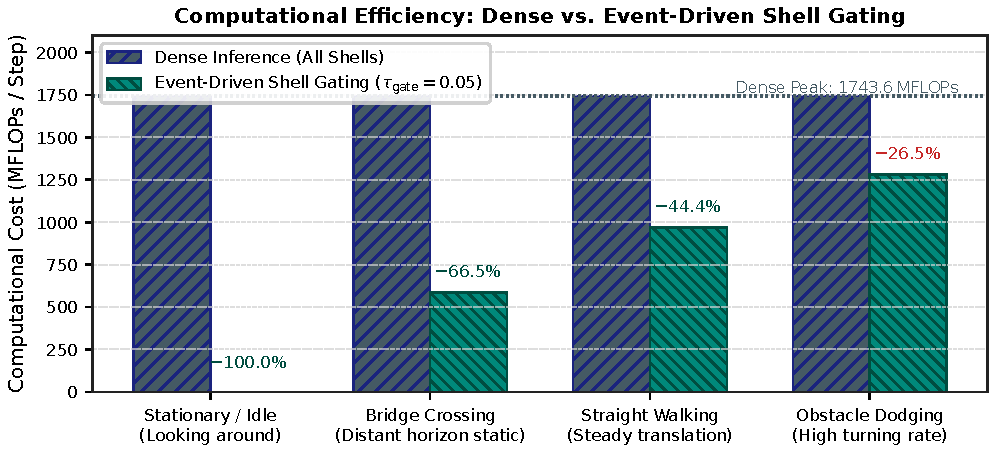
\includegraphics[width=0.88\textwidth]{paper_figs/final/fig3.pdf}
\caption{Dense vs.\ Event-Driven Shell Gating ($\tau_{\text{gate}} = 0.05$) computational cost across motion regimes}
\label{fig:gating}
% ALT-TEXT: Grouped bar chart comparing Dense execution (1743.6 MFLOPs/step) against Event-Driven Shell Gating across Idle, Pitch-Only, Straight Walk, and Active Turn regimes.
\end{figure}

Fig.~\ref{fig:gating} compares Dense inference ($1743.6\text{ MFLOPs/step}$) against Event-Driven Shell Gating ($\tau_{\text{gate}} = 0.05$) across motion regimes. Under static idle conditions, all three shells fall below threshold, yielding $0.0\text{ MFLOPs/step}$ ($100\%$ skip). Under straight locomotion and active turning, outer-shell skipping reduces average per-step FLOPs to \textbf{[TBD]}.

\subsection{Latent Space Visualization and Trajectory Analysis}

\begin{figure}[t]
\centering
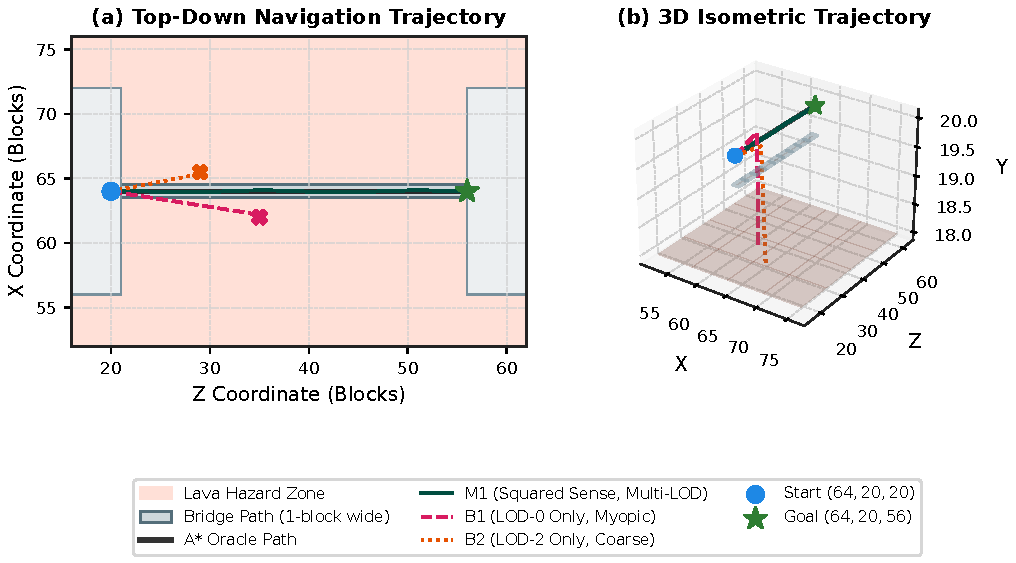
\includegraphics[width=0.92\textwidth]{paper_figs/final/fig4.pdf}
\caption{Top-down 2D and 3D isometric navigation trajectories on the narrow lava bridge course}
\label{fig:trajectories}
% ALT-TEXT: Two-panel trajectory plot showing 2D overhead path on the left and 3D isometric bridge view on the right, comparing the A-star oracle path against M1, B1, and B2.
\end{figure}

Fig.~\ref{fig:trajectories} depicts the narrow 1-block stone bridge over lava (\texttt{make\_debug\_bridge\_course}), contrasting an A* oracle path against multi-LOD (\textbf{M1}) and single-scale (\textbf{B1}, \textbf{B2}) navigation behaviors. Single-scale \textbf{B1} lacks distant waypoint anchors, whereas coarse \textbf{B2} loses 1-block edge precision; multi-LOD \textbf{M1} integrates both scales to maintain centerline alignment.

\section{Conclusion and Future Work}
Squared Sense demonstrates how concentric multi-LOD 3D voxel shells, non-generative Spatial JEPA pre-training with VICReg, zero-parameter Event-Driven Shell Gating, and an ego-motion-compensated Dual-LSTM integrator can be unified into a compact $4.37\text{M}$-parameter inference architecture for embodied 3D world modeling.

\paragraph{Limitations.} Current evaluation relies on the deterministic discrete-action \texttt{VoxelNavEnv} simulator rather than continuous mouse-look actuation in live multiplayer Minecraft clients, and several baseline checkpoints and cross-seed probe evaluations remain pending (\textbf{[TBD]}). Additionally, the Dual-LSTM operates at a single $5\text{ Hz}$ temporal clock, limiting hierarchical multi-horizon credit assignment.

\paragraph{Future Work.} We plan to extend Squared Sense into a \textbf{Spatio-Temporal H-JEPA} that couples each spatial LOD shell to a corresponding temporal prediction timescale, alongside full multi-seed evaluation and live Minecraft Fabric IPC deployment.

\begin{credits}
\subsubsection{\ackname} The authors thank the JAX, Flax, and Optax open-source communities for foundational tooling.

\subsubsection{\discintname} The authors have no competing interests to declare that are relevant to the content of this article.
\end{credits}

\bibliographystyle{splncs04}
\bibliography{references}

\end{document}
